% Options for packages loaded elsewhere
\PassOptionsToPackage{unicode}{hyperref}
\PassOptionsToPackage{hyphens}{url}
%
\documentclass[
]{article}
\usepackage{amsmath,amssymb}
\usepackage{lmodern}
\usepackage{ifxetex,ifluatex}
\ifnum 0\ifxetex 1\fi\ifluatex 1\fi=0 % if pdftex
  \usepackage[T1]{fontenc}
  \usepackage[utf8]{inputenc}
  \usepackage{textcomp} % provide euro and other symbols
\else % if luatex or xetex
  \usepackage{unicode-math}
  \defaultfontfeatures{Scale=MatchLowercase}
  \defaultfontfeatures[\rmfamily]{Ligatures=TeX,Scale=1}
\fi
% Use upquote if available, for straight quotes in verbatim environments
\IfFileExists{upquote.sty}{\usepackage{upquote}}{}
\IfFileExists{microtype.sty}{% use microtype if available
  \usepackage[]{microtype}
  \UseMicrotypeSet[protrusion]{basicmath} % disable protrusion for tt fonts
}{}
\makeatletter
\@ifundefined{KOMAClassName}{% if non-KOMA class
  \IfFileExists{parskip.sty}{%
    \usepackage{parskip}
  }{% else
    \setlength{\parindent}{0pt}
    \setlength{\parskip}{6pt plus 2pt minus 1pt}}
}{% if KOMA class
  \KOMAoptions{parskip=half}}
\makeatother
\usepackage{xcolor}
\IfFileExists{xurl.sty}{\usepackage{xurl}}{} % add URL line breaks if available
\IfFileExists{bookmark.sty}{\usepackage{bookmark}}{\usepackage{hyperref}}
\hypersetup{
  pdftitle={Clase 2: Trabajo práctico LaLonde (1996)},
  pdfauthor={Arturo Maldonado},
  hidelinks,
  pdfcreator={LaTeX via pandoc}}
\urlstyle{same} % disable monospaced font for URLs
\usepackage[margin=1in]{geometry}
\usepackage{color}
\usepackage{fancyvrb}
\newcommand{\VerbBar}{|}
\newcommand{\VERB}{\Verb[commandchars=\\\{\}]}
\DefineVerbatimEnvironment{Highlighting}{Verbatim}{commandchars=\\\{\}}
% Add ',fontsize=\small' for more characters per line
\usepackage{framed}
\definecolor{shadecolor}{RGB}{248,248,248}
\newenvironment{Shaded}{\begin{snugshade}}{\end{snugshade}}
\newcommand{\AlertTok}[1]{\textcolor[rgb]{0.94,0.16,0.16}{#1}}
\newcommand{\AnnotationTok}[1]{\textcolor[rgb]{0.56,0.35,0.01}{\textbf{\textit{#1}}}}
\newcommand{\AttributeTok}[1]{\textcolor[rgb]{0.77,0.63,0.00}{#1}}
\newcommand{\BaseNTok}[1]{\textcolor[rgb]{0.00,0.00,0.81}{#1}}
\newcommand{\BuiltInTok}[1]{#1}
\newcommand{\CharTok}[1]{\textcolor[rgb]{0.31,0.60,0.02}{#1}}
\newcommand{\CommentTok}[1]{\textcolor[rgb]{0.56,0.35,0.01}{\textit{#1}}}
\newcommand{\CommentVarTok}[1]{\textcolor[rgb]{0.56,0.35,0.01}{\textbf{\textit{#1}}}}
\newcommand{\ConstantTok}[1]{\textcolor[rgb]{0.00,0.00,0.00}{#1}}
\newcommand{\ControlFlowTok}[1]{\textcolor[rgb]{0.13,0.29,0.53}{\textbf{#1}}}
\newcommand{\DataTypeTok}[1]{\textcolor[rgb]{0.13,0.29,0.53}{#1}}
\newcommand{\DecValTok}[1]{\textcolor[rgb]{0.00,0.00,0.81}{#1}}
\newcommand{\DocumentationTok}[1]{\textcolor[rgb]{0.56,0.35,0.01}{\textbf{\textit{#1}}}}
\newcommand{\ErrorTok}[1]{\textcolor[rgb]{0.64,0.00,0.00}{\textbf{#1}}}
\newcommand{\ExtensionTok}[1]{#1}
\newcommand{\FloatTok}[1]{\textcolor[rgb]{0.00,0.00,0.81}{#1}}
\newcommand{\FunctionTok}[1]{\textcolor[rgb]{0.00,0.00,0.00}{#1}}
\newcommand{\ImportTok}[1]{#1}
\newcommand{\InformationTok}[1]{\textcolor[rgb]{0.56,0.35,0.01}{\textbf{\textit{#1}}}}
\newcommand{\KeywordTok}[1]{\textcolor[rgb]{0.13,0.29,0.53}{\textbf{#1}}}
\newcommand{\NormalTok}[1]{#1}
\newcommand{\OperatorTok}[1]{\textcolor[rgb]{0.81,0.36,0.00}{\textbf{#1}}}
\newcommand{\OtherTok}[1]{\textcolor[rgb]{0.56,0.35,0.01}{#1}}
\newcommand{\PreprocessorTok}[1]{\textcolor[rgb]{0.56,0.35,0.01}{\textit{#1}}}
\newcommand{\RegionMarkerTok}[1]{#1}
\newcommand{\SpecialCharTok}[1]{\textcolor[rgb]{0.00,0.00,0.00}{#1}}
\newcommand{\SpecialStringTok}[1]{\textcolor[rgb]{0.31,0.60,0.02}{#1}}
\newcommand{\StringTok}[1]{\textcolor[rgb]{0.31,0.60,0.02}{#1}}
\newcommand{\VariableTok}[1]{\textcolor[rgb]{0.00,0.00,0.00}{#1}}
\newcommand{\VerbatimStringTok}[1]{\textcolor[rgb]{0.31,0.60,0.02}{#1}}
\newcommand{\WarningTok}[1]{\textcolor[rgb]{0.56,0.35,0.01}{\textbf{\textit{#1}}}}
\usepackage{longtable,booktabs,array}
\usepackage{calc} % for calculating minipage widths
% Correct order of tables after \paragraph or \subparagraph
\usepackage{etoolbox}
\makeatletter
\patchcmd\longtable{\par}{\if@noskipsec\mbox{}\fi\par}{}{}
\makeatother
% Allow footnotes in longtable head/foot
\IfFileExists{footnotehyper.sty}{\usepackage{footnotehyper}}{\usepackage{footnote}}
\makesavenoteenv{longtable}
\usepackage{graphicx}
\makeatletter
\def\maxwidth{\ifdim\Gin@nat@width>\linewidth\linewidth\else\Gin@nat@width\fi}
\def\maxheight{\ifdim\Gin@nat@height>\textheight\textheight\else\Gin@nat@height\fi}
\makeatother
% Scale images if necessary, so that they will not overflow the page
% margins by default, and it is still possible to overwrite the defaults
% using explicit options in \includegraphics[width, height, ...]{}
\setkeys{Gin}{width=\maxwidth,height=\maxheight,keepaspectratio}
% Set default figure placement to htbp
\makeatletter
\def\fps@figure{htbp}
\makeatother
\setlength{\emergencystretch}{3em} % prevent overfull lines
\providecommand{\tightlist}{%
  \setlength{\itemsep}{0pt}\setlength{\parskip}{0pt}}
\setcounter{secnumdepth}{-\maxdimen} % remove section numbering
\ifluatex
  \usepackage{selnolig}  % disable illegal ligatures
\fi

\title{Clase 2: Trabajo práctico LaLonde (1996)}
\author{Arturo Maldonado}
\date{3/22/2021}

\begin{document}
\maketitle

\hypertarget{medidas-de-tendencia-central}{%
\section{Medidas de tendencia
central}\label{medidas-de-tendencia-central}}

\begin{itemize}
\item
  Resumen de un conjunto de datos.
\item
  Se resume mediante un valor ``representativo.''
\item
  Cada observación se puede comparar con este valor de resumen. Se puede
  estar por debajo o por encima de este valor.
\end{itemize}

\hypertarget{moda}{%
\subsection{Moda}\label{moda}}

\begin{itemize}
\item
  Valor mas frecuente de un conjunto de datos
\item
  Es apropiada para todo tipo de datos
\item
  Se puede observar directamente en una tabla de distribución de
  frecuencias.
\end{itemize}

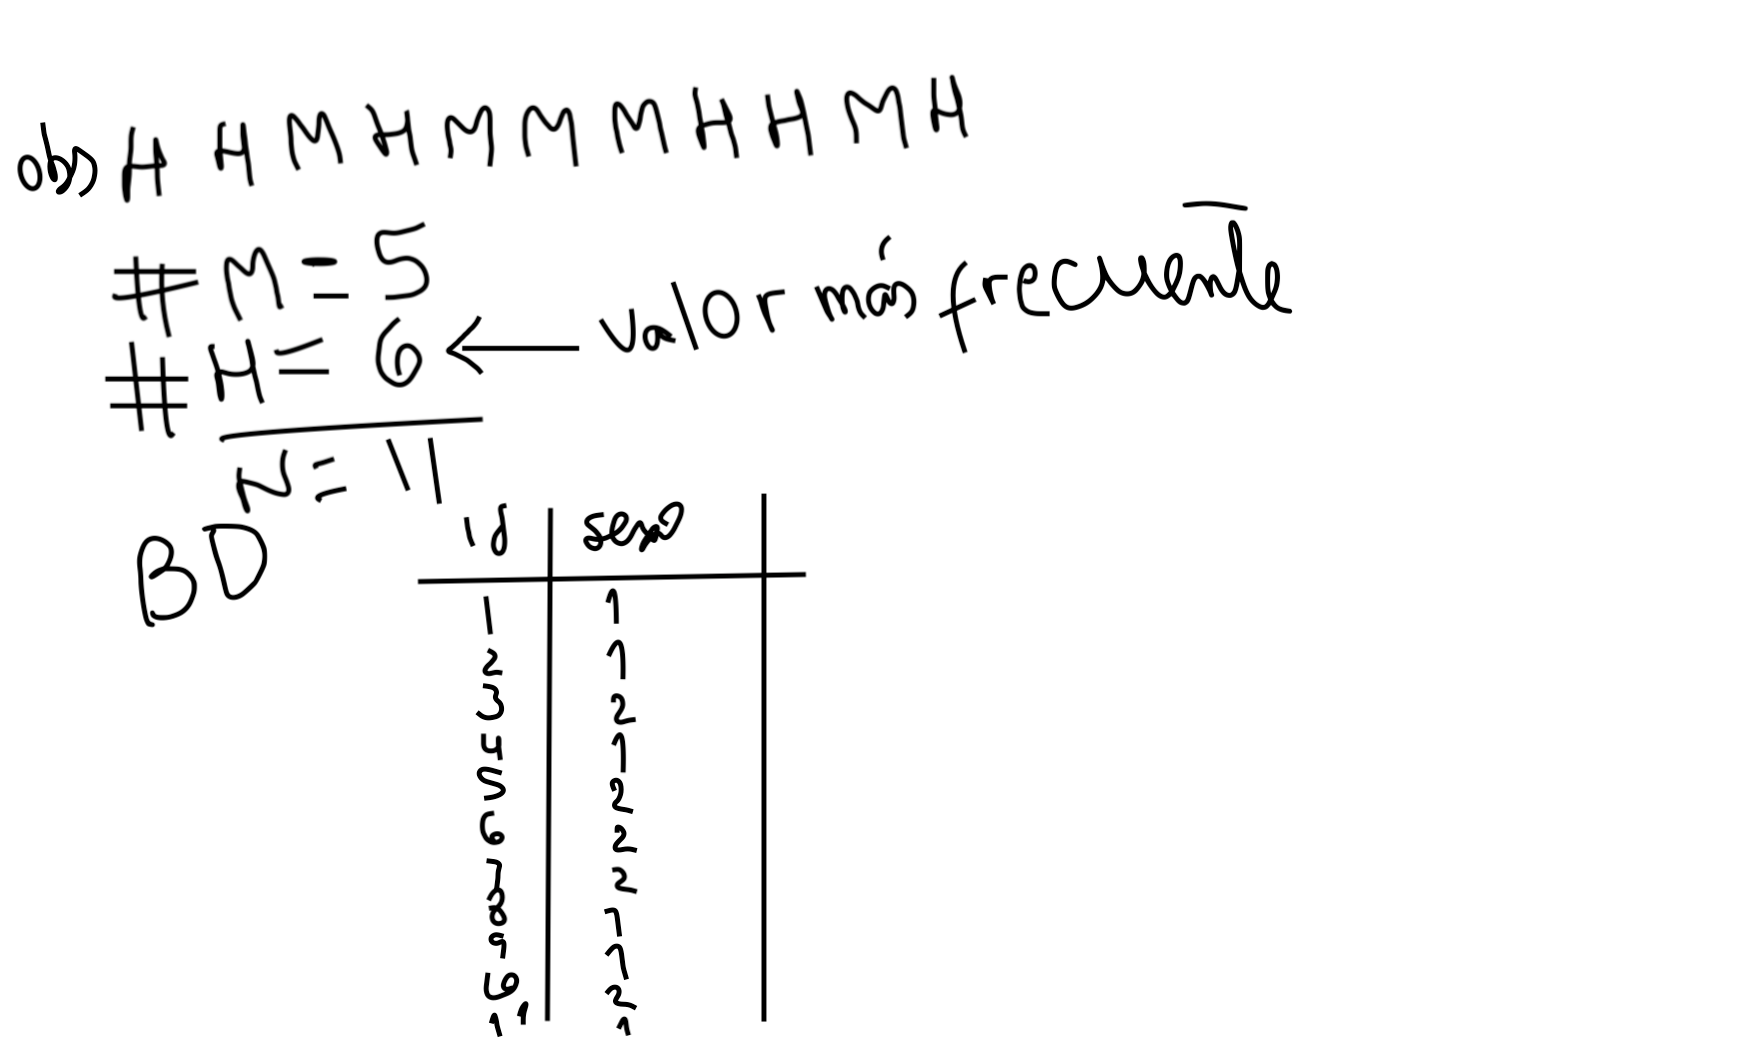
\includegraphics[width=6.13542in,height=\textheight]{Captura de Pantalla 2021-04-02 a la(s) 12.12.02.png}

\hypertarget{mediana}{%
\subsection{Mediana}\label{mediana}}

\begin{itemize}
\tightlist
\item
  El valor de la observación central de un conjunto de datos ordenados
  de menor a mayor.
\end{itemize}

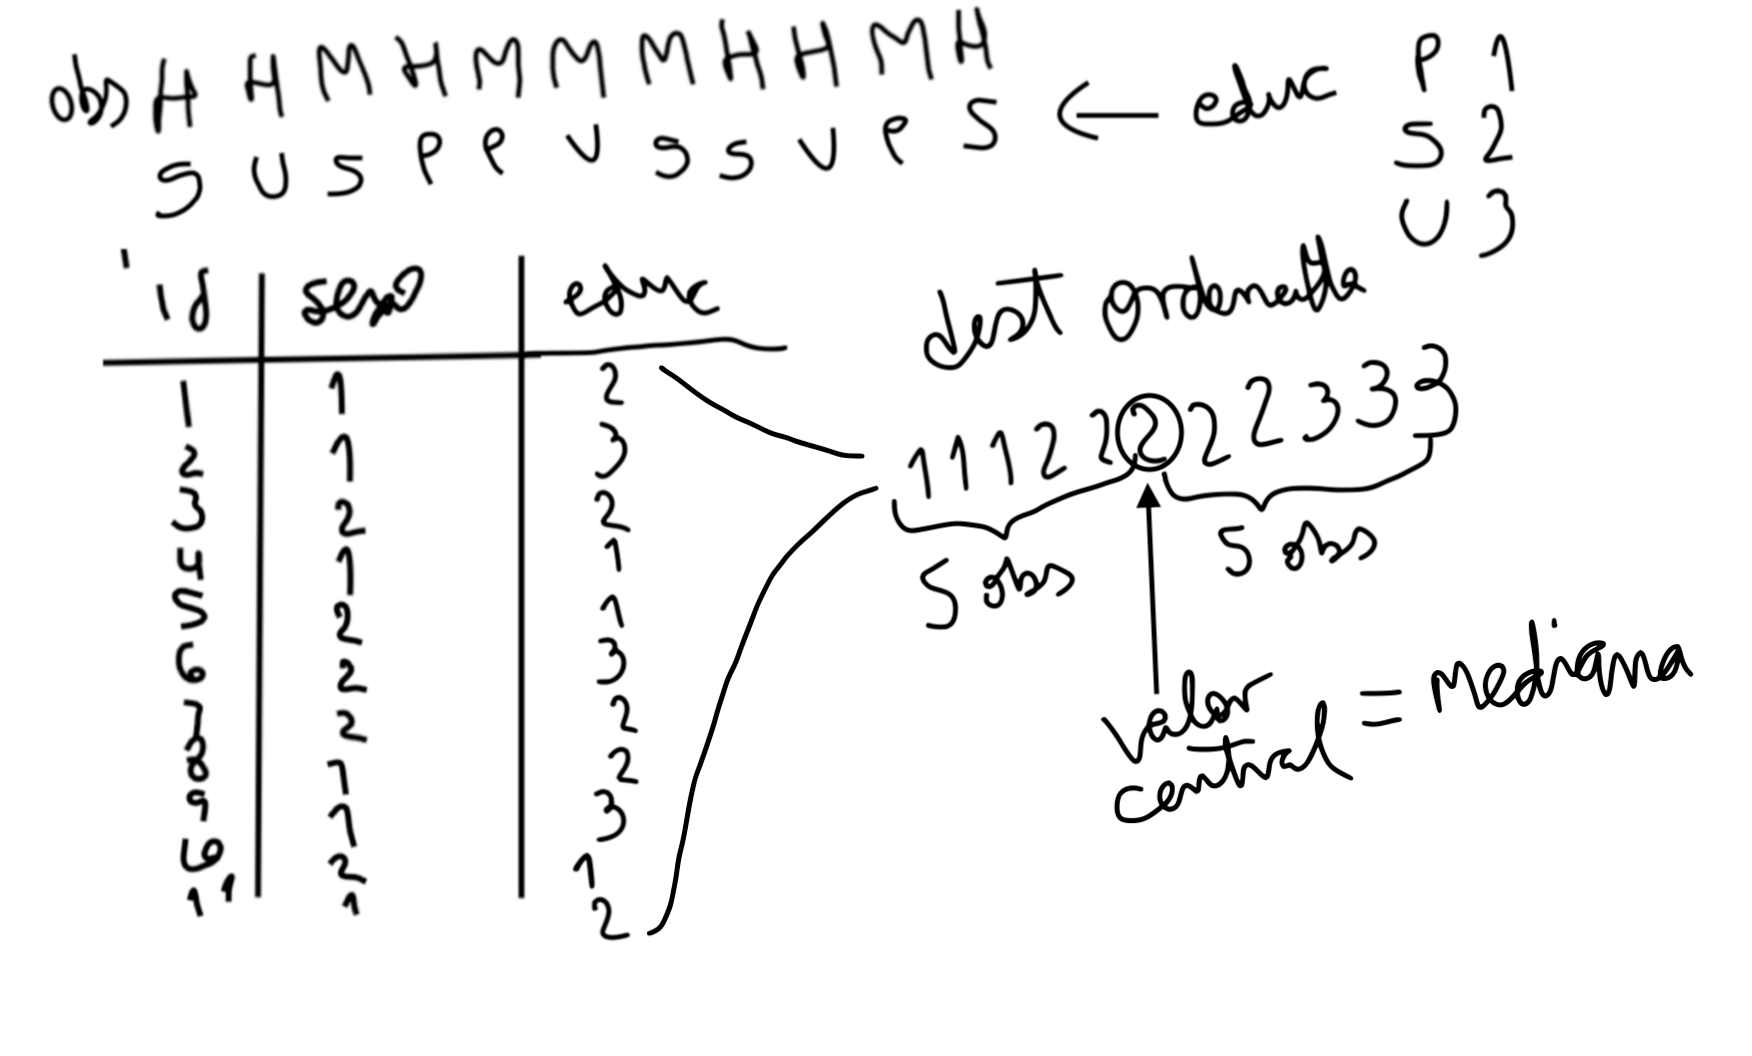
\includegraphics[width=6.15625in,height=\textheight]{mediana.png}

\hypertarget{media}{%
\subsection{Media}\label{media}}

\begin{itemize}
\item
  Medida más conocida y ``útil.''
\item
  Suma del valor de las observaciones dividida entre el número de
  observaciones
\end{itemize}

\[
\sum \frac{x_i} {n} = \frac{(x_1 + x_2 +x_3 +...+ x_n)} {n}
\]

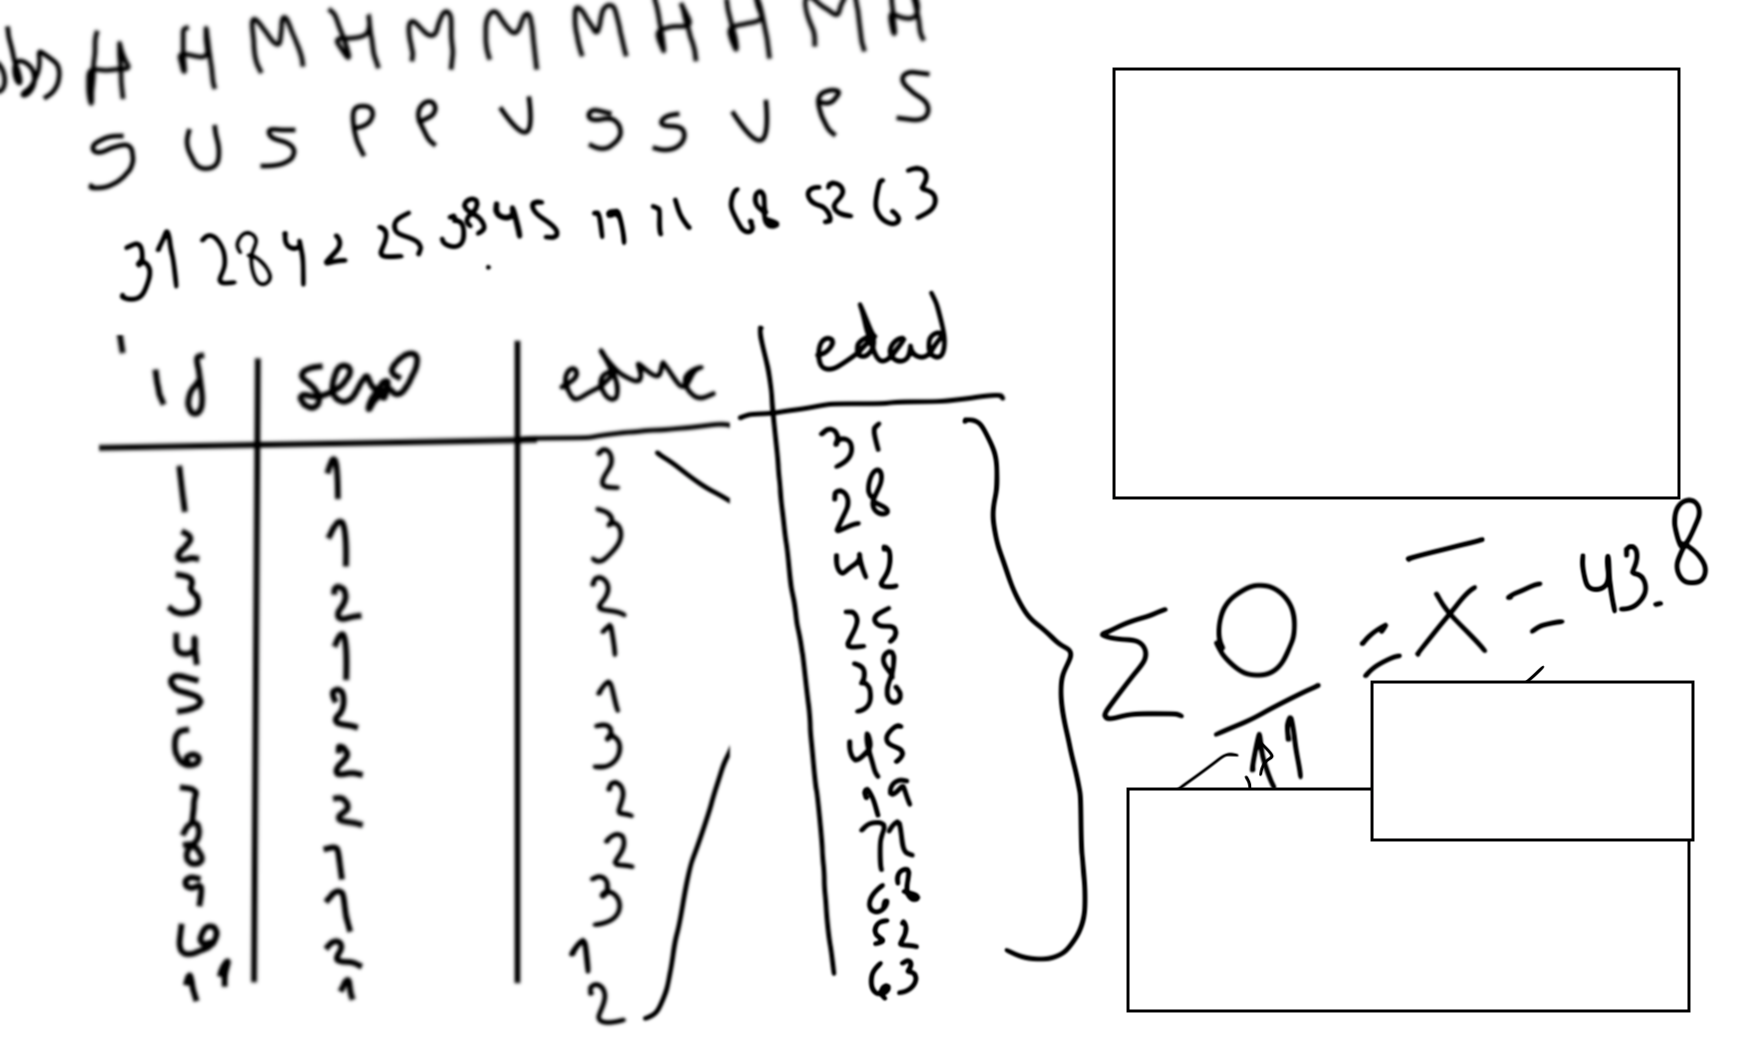
\includegraphics[width=6.1875in,height=\textheight]{media.png}

\hypertarget{resumen}{%
\subsection{Resumen}\label{resumen}}

\begin{longtable}[]{@{}
  >{\raggedright\arraybackslash}p{(\columnwidth - 6\tabcolsep) * \real{0.14}}
  >{\centering\arraybackslash}p{(\columnwidth - 6\tabcolsep) * \real{0.17}}
  >{\centering\arraybackslash}p{(\columnwidth - 6\tabcolsep) * \real{0.17}}
  >{\centering\arraybackslash}p{(\columnwidth - 6\tabcolsep) * \real{0.17}}@{}}
\toprule
TC & Nominales & Ordinales & Numéricas \\
\midrule
\endhead
Moda & Sí & Sí & Sí \\
Mediana & No & Sí & Sí \\
Media & No & No & Sí \\
\bottomrule
\end{longtable}

\begin{itemize}
\item
  Moda aplica para cualquier tipo de variable, pero menos útil.
\item
  Media aplica solo para variables numéricas, pero más útil.
\end{itemize}

\hypertarget{medidas-de-dispersiuxf3n}{%
\section{Medidas de dispersión}\label{medidas-de-dispersiuxf3n}}

\begin{itemize}
\item
  Describir la centralidad no es suficiente. Dos distribuciones pueden
  tener la misma medida de tendencia central, pero diferentes
  realidades.
\item
  Ejemplo: distribución de puntaje en área matemática de prueba PISA
  aplicada en 2 países pueden tener la misma media, pero diferente
  forma.
\item
  ¿Cómo describiría las diferencias entre el País A y el País B?
\end{itemize}

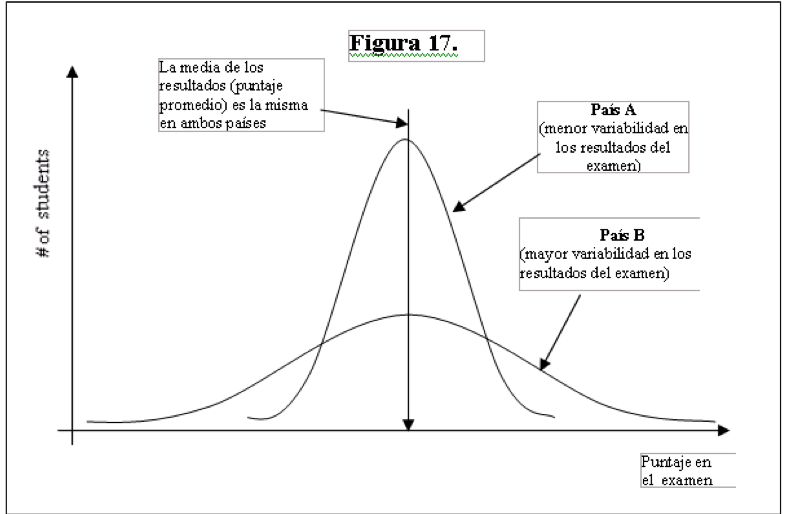
\includegraphics[width=6.57292in,height=\textheight]{distr.png}

\hypertarget{rango}{%
\subsection{Rango}\label{rango}}

\begin{itemize}
\item
  Diferencia entre el valor máximo y el mínimo. En ejemplo de edades:
  68-19 = 49 años.
\item
  No un una medida muy útil.
\end{itemize}

\hypertarget{rango-intercuartil}{%
\subsection{Rango intercuartil}\label{rango-intercuartil}}

\begin{itemize}
\tightlist
\item
  Se verá cuando se vean percentiles.
\end{itemize}

\hypertarget{desviaciuxf3n-estuxe1ndar}{%
\subsection{Desviación estándar}\label{desviaciuxf3n-estuxe1ndar}}

\begin{itemize}
\item
  Cada observación está a una ``distancia'' de la media. Esta distancia
  se llama desviación \((x_i-\bar{x})\)
\item
  Observaciones por encima de la media tendrán desviaciones positivas.
  Observaciones por debajo de la media tendrán desviaciones negativas.
\item
  No se puede calcular un promedio de desviaciones porque valores
  positivos se cancelan con negativos.
\item
  Se eleva al cuadrado las observaciones para que todas sean positivas.
  Se promedian esas desviaciones al cuadrado.
\item
  La desviación estándar es la raíz cuadrada de ese promedio de
  desviaciones al cuadrado.
\item
  Se divide entre n-1 por un tema técnico.
\end{itemize}

\[
\sum \frac{(x_i-\bar{x})^2} {n-1} 
\]

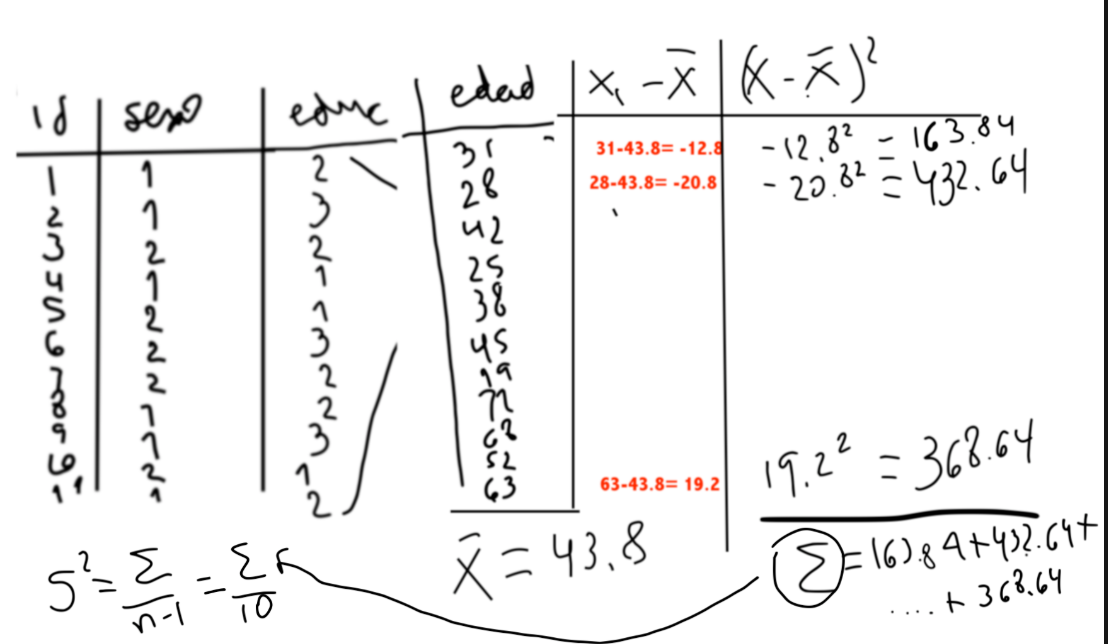
\includegraphics[width=6.60417in,height=\textheight]{desviacion.png}

\hypertarget{paper-evaluating-the-econometric-evaluations-of-training-programs-with-experimental-data}{%
\section{Paper ``Evaluating the Econometric Evaluations of Training
Programs with Experimental
Data''}\label{paper-evaluating-the-econometric-evaluations-of-training-programs-with-experimental-data}}

Pregunta: ¿tiene un efecto los programas de entrenamiento en la
empleabilidad?

Supuesto: entrenando a trabajadores que no tienen las habilidades
básicas hará que se muevan en el mercado laboral, dándoles experiencia
laboral y consejería. Se trata de un programa estatal que garantiza un
trabajo entre 9 a 18 meses. Luego de este periodo eran forzados a
encontrar un trabajo regular.

Metodología: evaluación experimental. Un grupo fue parte del programa.
Otro grupo comparable no fue parte del programa. Se recolectó una línea
de base con información de ingresos y datos sociodemográficos. Luego se
hizo recojo de información de seguimiento.

Variable de éxito: cambio en los ingresos.

\hypertarget{leyendo-la-base-de-datos-en-r}{%
\section{Leyendo la base de datos en
R}\label{leyendo-la-base-de-datos-en-r}}

\begin{Shaded}
\begin{Highlighting}[]
\NormalTok{LL }\OtherTok{\textless{}{-}} \FunctionTok{read.csv}\NormalTok{(}\StringTok{"\textasciitilde{}/OneDrive {-} Vanderbilt/A Cursos/Estadistica\_1/Sesión 2 Centralidad Dispersión/Caso/LL.csv"}\NormalTok{)}
\end{Highlighting}
\end{Shaded}

\hypertarget{variables-en-la-base-de-datos}{%
\section{Variables en la base de
datos}\label{variables-en-la-base-de-datos}}

\begin{itemize}
\tightlist
\item
  treated: variable dummy si el participante recibió el tratamiento (1)
  o no (0)
\item
  age: edad
\item
  education: años de educación
\item
  black: variable dummy si el participante es Afroamericano
\item
  married: variable dummy si el participante es casado
\item
  nodegree: variable dummy de no tener estudios secundarios completos
  (high school)
\item
  re74: ingresos reales en 1974
\item
  re75: ingresos reales en 1975
\item
  re78: ingresos reales en 1978
\item
  hispanic: variable dummy si el participantes es hispano
\item
  u74: variable dummy si era desempleado en 1974
\item
  u75: variable dummy si era desempleado en 1975
\end{itemize}

\hypertarget{medidas-de-tendencia-central-1}{%
\section{Medidas de tendencia
central}\label{medidas-de-tendencia-central-1}}

\hypertarget{media-1}{%
\subsection{Media}\label{media-1}}

¿Cual es la media de ingresos de los participantes antes de entrar al
estudio? Ojo que algunos de ellos pueden haber entrado al programa y
otros ser parte del grupo de comparación.

\begin{Shaded}
\begin{Highlighting}[]
\FunctionTok{mean}\NormalTok{(LL}\SpecialCharTok{$}\NormalTok{re74)}
\end{Highlighting}
\end{Shaded}

\begin{verbatim}
## [1] 3630.738
\end{verbatim}

Aparentemente, el ingreso de los participantes del estudio en la línea
de base es bastante bueno. Pero, es necesario hacer ver si ese dato
refleja la ``realidad'' de los ingresos del conjunto de participantes
del estudio. Una manera de analizar eso, es ver la distribución de
respuestas de forma gráfica, por ejemplo, usando un histograma. En este
gráfico, además, se puede incluir una línea que marque el punto de la
media.

\begin{Shaded}
\begin{Highlighting}[]
\FunctionTok{hist}\NormalTok{(LL}\SpecialCharTok{$}\NormalTok{re74)}
\FunctionTok{abline}\NormalTok{(}\AttributeTok{v=}\FunctionTok{mean}\NormalTok{(LL}\SpecialCharTok{$}\NormalTok{re74), }\AttributeTok{col=}\StringTok{"red"}\NormalTok{)}
\end{Highlighting}
\end{Shaded}

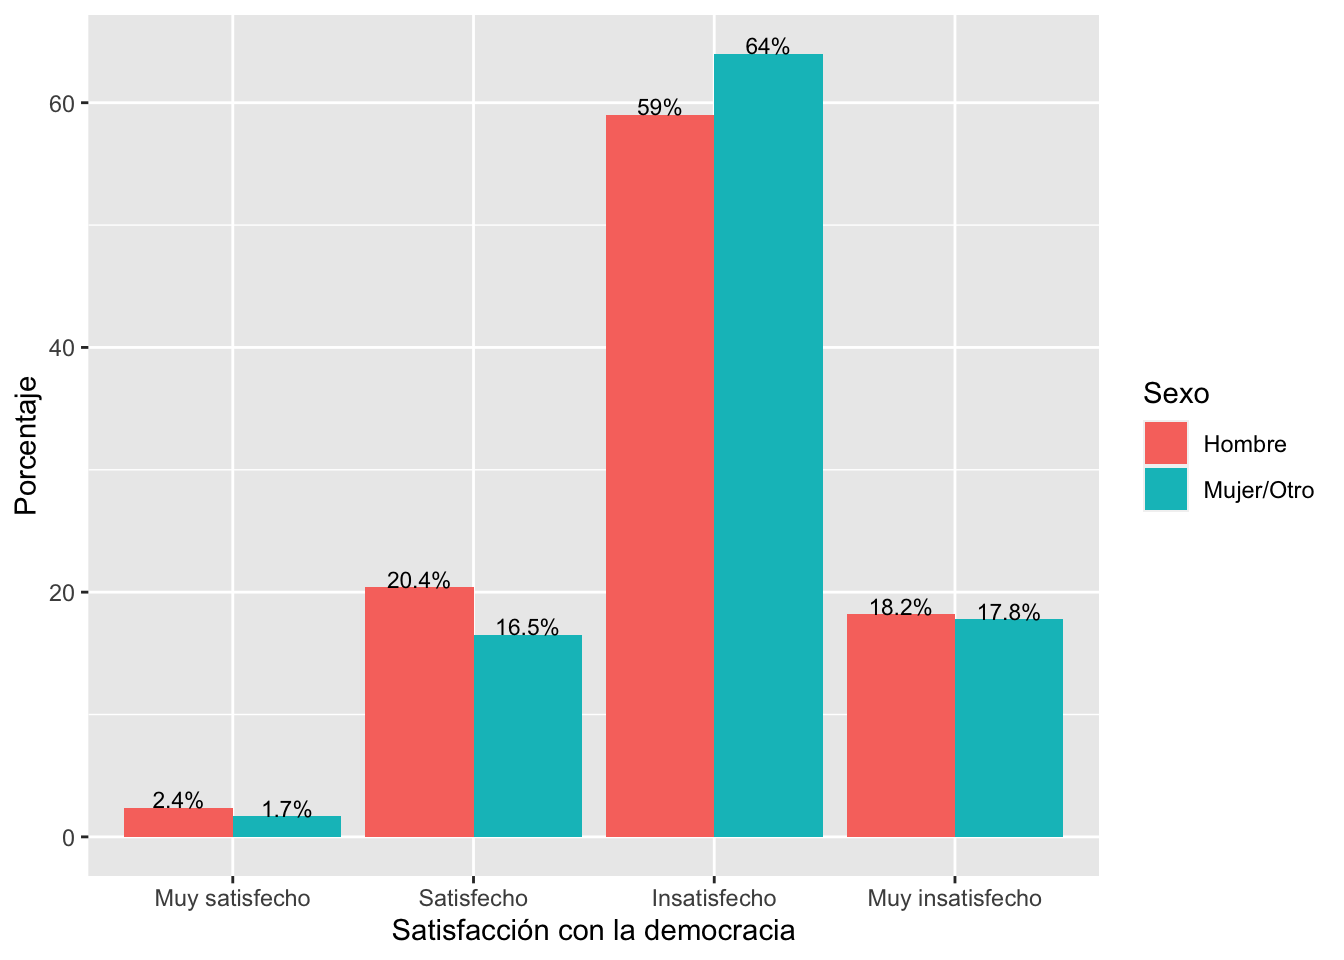
\includegraphics{clase2_files/figure-latex/unnamed-chunk-1-1.pdf}

Como se observa, la distribución de esta variable está sesgada hacia los
valores altos de la variable. ¿Qué pasa con la media en estas
situaciones?

\hypertarget{mediana-1}{%
\subsection{Mediana}\label{mediana-1}}

Para estos casos, se tiene otra medida de tendencia central, la mediana.
La mediana es el punto medio de un conjunto de datos ordenados. Por
ejemplo, si tengo 5 personas con los siguientes ingresos ordenados: 800,
1200, 1500, 3000, 5000. La mediana es el ingreso de la persona que está
al medio de la fila ordenada, es decir, la persona en la posición 3. La
mediana sería 1500 soles. La media de estas 5 observaciones sería 2300
soles. Si se quisiera ``encontrar'' la mediana en la base de datos, ¿qué
se debería hacer? ¿Si son 722 observaciones, cuál es el punto medio?

La fila sería de observación 1\ldots..411 / 412\ldots\ldots822 La
mediana sería el promedio simple del valor del ingreso que tiene la
persona ubicada en la posición 411 (823.2544) y del de la posición 412
(824.3886).

Para calcular la mediana del grupo del estudio, se usa.

\begin{Shaded}
\begin{Highlighting}[]
\FunctionTok{median}\NormalTok{(LL}\SpecialCharTok{$}\NormalTok{re74)}
\end{Highlighting}
\end{Shaded}

\begin{verbatim}
## [1] 823.8215
\end{verbatim}

Como se observa la mediana es mucho menor que la media y, en este caso,
es un mejor resumen de la ``realidad'' del conjunto de ingresos de los
participantes en este estudio.

¿Qué pasa si en mi ejemplo de la fila, la última persona que gana 5000
recibe un súper aumento y pasa a ganar 15000 soles. ¿Cambia la media?
¿Cambia la mediana?

\hypertarget{resumen-de-una-variable}{%
\subsection{Resumen de una variable}\label{resumen-de-una-variable}}

Si se quisiera ver la media y la mediana con un solo comando, se puede
usar \texttt{summary}.

\begin{Shaded}
\begin{Highlighting}[]
\FunctionTok{summary}\NormalTok{(LL}\SpecialCharTok{$}\NormalTok{re74)}
\end{Highlighting}
\end{Shaded}

\begin{verbatim}
##    Min. 1st Qu.  Median    Mean 3rd Qu.    Max. 
##     0.0     0.0   823.8  3630.7  5211.8 39570.7
\end{verbatim}

Se observa claramente que la media es mucho mayor que la mediana. Lo
cual también se puede graficar

\begin{Shaded}
\begin{Highlighting}[]
\FunctionTok{hist}\NormalTok{(LL}\SpecialCharTok{$}\NormalTok{re74, }\AttributeTok{breaks =} \DecValTok{15}\NormalTok{)}
\FunctionTok{abline}\NormalTok{(}\AttributeTok{v=}\FunctionTok{mean}\NormalTok{(LL}\SpecialCharTok{$}\NormalTok{re74), }\AttributeTok{col=}\StringTok{"red"}\NormalTok{)}
\FunctionTok{abline}\NormalTok{(}\AttributeTok{v=}\FunctionTok{median}\NormalTok{(LL}\SpecialCharTok{$}\NormalTok{re74), }\AttributeTok{col=}\StringTok{"blue"}\NormalTok{)}
\end{Highlighting}
\end{Shaded}

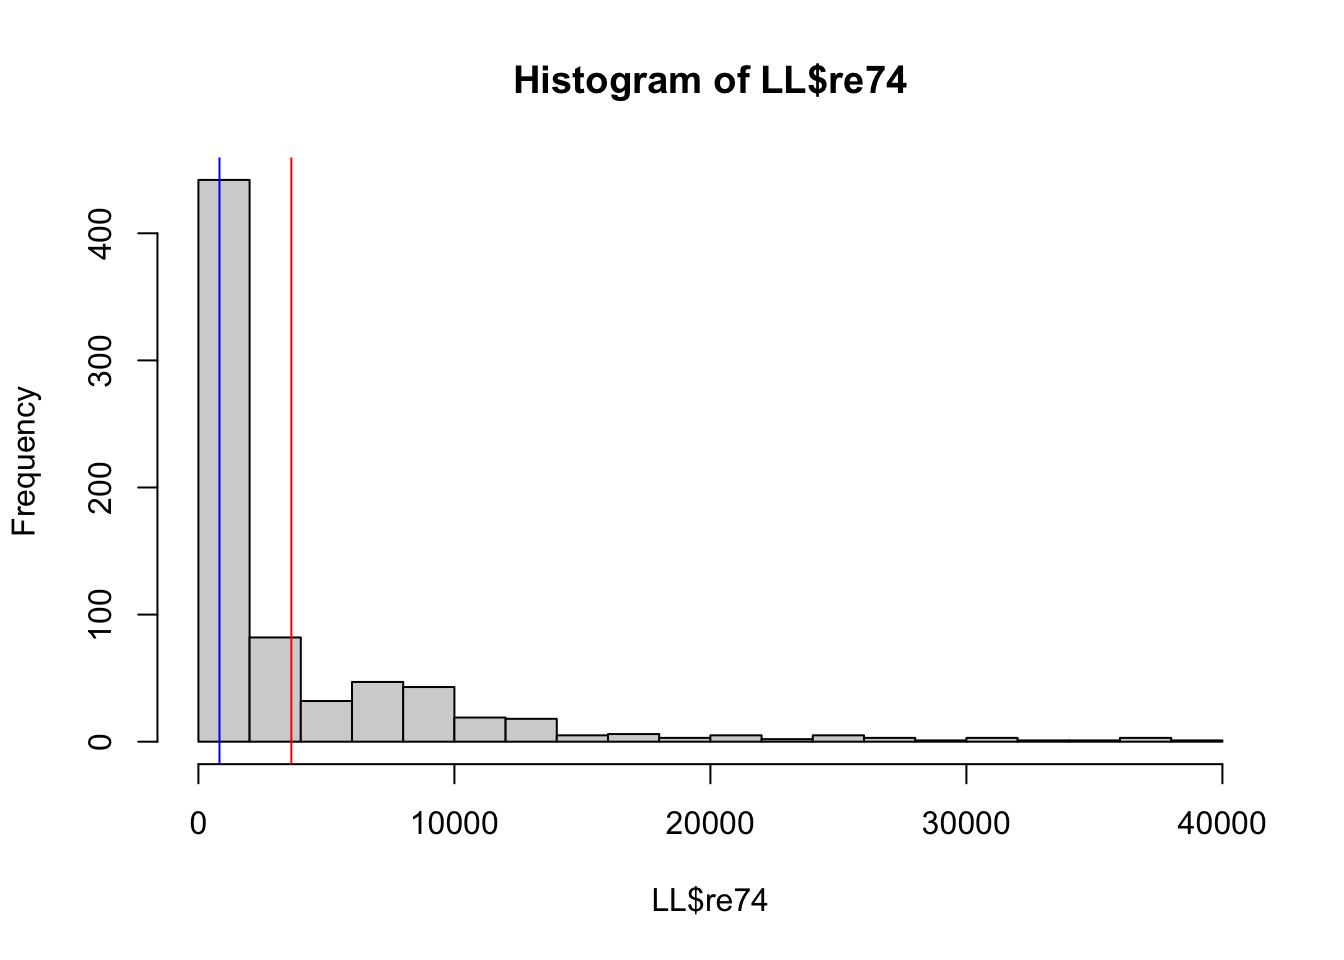
\includegraphics{clase2_files/figure-latex/unnamed-chunk-3-1.pdf}

Con el comando \texttt{summary}se puede ver que la mediana aparece como
un caso particular de los cuartiles. Los cuartiles dividen a la
distribución en grupos de igual tamaño. Así como la mediana divide a la
``fila ordenada'' en 2 grupos, cada uno con 411 observaciones, los
cuartiles dividen la distribución en 4 grupos, cada uno con el 25\% del
total de observaciones (180.5 observaciones). ¿Qué significa que el
Min=0? ¿Qué significa 1st Qu = 0? ¿Median a qué porcentaje corresponde?
¿3rd Qu a qué porcentaje corresponde? ¿Qué significa Max? ¿Máximo
observado puede ser atípico?

\hypertarget{gruxe1fico-de-cajas}{%
\subsection{Gráfico de cajas}\label{gruxe1fico-de-cajas}}

Una forma de graficar los cuartiles es mediante el gráfico de cajas o
boxplot (ver ppt). Este gráfico muestra una caja central y dos bigotes.
El gráfico para la variable ingresos de la línea de base es:

\begin{Shaded}
\begin{Highlighting}[]
\FunctionTok{boxplot}\NormalTok{(LL}\SpecialCharTok{$}\NormalTok{re74)}
\end{Highlighting}
\end{Shaded}

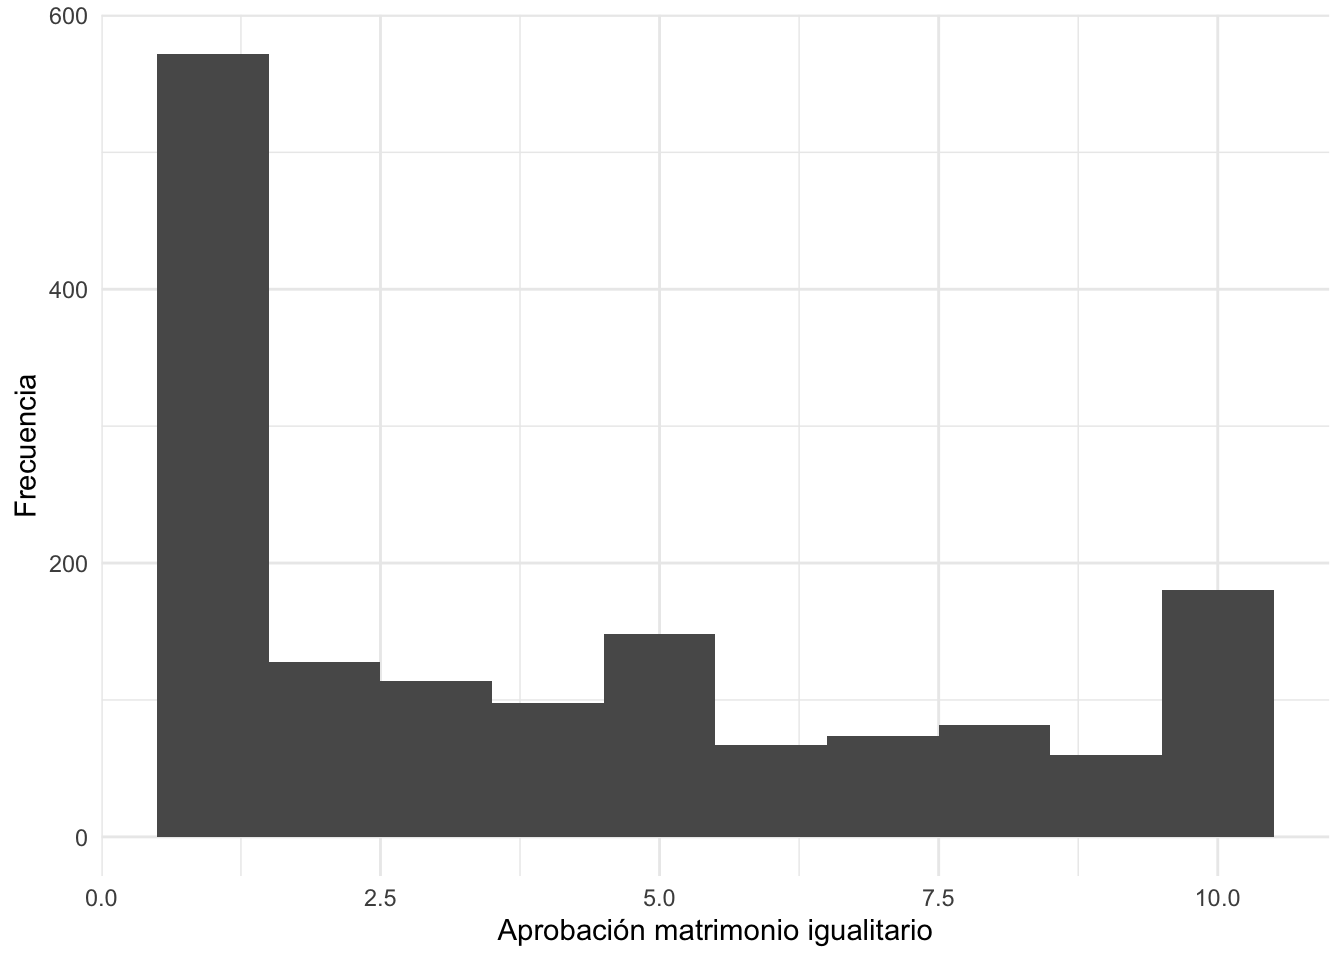
\includegraphics{clase2_files/figure-latex/unnamed-chunk-4-1.pdf}

¿Por qué no se muestra el bigote inferior? ¿Qué significan los puntos
superiores?

Los cuartiles son una posibilidad de los percentiles. Una opción
bastante usada es los deciles.

\begin{Shaded}
\begin{Highlighting}[]
\FunctionTok{quantile}\NormalTok{(LL}\SpecialCharTok{$}\NormalTok{re74)}
\end{Highlighting}
\end{Shaded}

\begin{verbatim}
##         0%        25%        50%        75%       100% 
##     0.0000     0.0000   823.8215  5211.7946 39570.6797
\end{verbatim}

\begin{Shaded}
\begin{Highlighting}[]
\FunctionTok{quantile}\NormalTok{(LL}\SpecialCharTok{$}\NormalTok{re74, }\FunctionTok{c}\NormalTok{(}\DecValTok{0}\NormalTok{,.}\DecValTok{1}\NormalTok{,.}\DecValTok{2}\NormalTok{,.}\DecValTok{3}\NormalTok{,.}\DecValTok{4}\NormalTok{,.}\DecValTok{5}\NormalTok{,.}\DecValTok{6}\NormalTok{,.}\DecValTok{7}\NormalTok{,.}\DecValTok{8}\NormalTok{,.}\DecValTok{9}\NormalTok{,}\DecValTok{1}\NormalTok{))}
\end{Highlighting}
\end{Shaded}

\begin{verbatim}
##         0%        10%        20%        30%        40%        50%        60% 
##     0.0000     0.0000     0.0000     0.0000     0.0000   823.8215  1837.2208 
##        70%        80%        90%       100% 
##  3343.5705  6651.6747 10393.2177 39570.6797
\end{verbatim}

\hypertarget{tablas-de-frecuencias}{%
\subsection{Tablas de frecuencias}\label{tablas-de-frecuencias}}

El ingreso descrito anteriormente es para toda la muestra. El estudio,
sin embargo, dividió a los participantes en 2 grupos: tratados y
control. ¿Cuántos hay en cada grupo?

\begin{Shaded}
\begin{Highlighting}[]
\FunctionTok{table}\NormalTok{(LL}\SpecialCharTok{$}\NormalTok{treated)}
\end{Highlighting}
\end{Shaded}

\begin{verbatim}
## 
##   0   1 
## 425 297
\end{verbatim}

La línea de base también recogió información sociodemográfica de los
participantes. En particular, nos interesa saber cuántos afroamericanos
hay en el grupo.

\begin{Shaded}
\begin{Highlighting}[]
\FunctionTok{table}\NormalTok{(LL}\SpecialCharTok{$}\NormalTok{black)}
\end{Highlighting}
\end{Shaded}

\begin{verbatim}
## 
##   0   1 
## 144 578
\end{verbatim}

Y sobre todo saber qué nivel educativo tienen.

\begin{Shaded}
\begin{Highlighting}[]
\FunctionTok{table}\NormalTok{(LL}\SpecialCharTok{$}\NormalTok{education)}
\end{Highlighting}
\end{Shaded}

\begin{verbatim}
## 
##   3   4   5   6   7   8   9  10  11  12  13  14  15  16 
##   1   6   5   7  15  62 110 162 195 122  23  11   2   1
\end{verbatim}

Las frecuencias absolutas no nos ayudan mucho, es mejor tener las
frecuencias relativas.

\begin{Shaded}
\begin{Highlighting}[]
\DecValTok{100}\SpecialCharTok{*}\FunctionTok{table}\NormalTok{(LL}\SpecialCharTok{$}\NormalTok{education)}\SpecialCharTok{/}\FunctionTok{sum}\NormalTok{(}\FunctionTok{table}\NormalTok{(LL}\SpecialCharTok{$}\NormalTok{education))}
\end{Highlighting}
\end{Shaded}

\begin{verbatim}
## 
##          3          4          5          6          7          8          9 
##  0.1385042  0.8310249  0.6925208  0.9695291  2.0775623  8.5872576 15.2354571 
##         10         11         12         13         14         15         16 
## 22.4376731 27.0083102 16.8975069  3.1855956  1.5235457  0.2770083  0.1385042
\end{verbatim}

O, se puede usar el comando \texttt{prop.table} que nos da la proporción
(en escala 0-1). Para reportar el porcentaje se multiplica por 100.

\begin{Shaded}
\begin{Highlighting}[]
\FunctionTok{prop.table}\NormalTok{(}\FunctionTok{table}\NormalTok{(LL}\SpecialCharTok{$}\NormalTok{education))}\SpecialCharTok{*}\DecValTok{100}
\end{Highlighting}
\end{Shaded}

\begin{verbatim}
## 
##          3          4          5          6          7          8          9 
##  0.1385042  0.8310249  0.6925208  0.9695291  2.0775623  8.5872576 15.2354571 
##         10         11         12         13         14         15         16 
## 22.4376731 27.0083102 16.8975069  3.1855956  1.5235457  0.2770083  0.1385042
\end{verbatim}

Esta variable se podría considerar como numérica, por lo que se podría
describir.

\begin{Shaded}
\begin{Highlighting}[]
\FunctionTok{summary}\NormalTok{(LL}\SpecialCharTok{$}\NormalTok{education)}
\end{Highlighting}
\end{Shaded}

\begin{verbatim}
##    Min. 1st Qu.  Median    Mean 3rd Qu.    Max. 
##    3.00    9.00   10.00   10.27   11.00   16.00
\end{verbatim}

Y se podría graficar

\begin{Shaded}
\begin{Highlighting}[]
\FunctionTok{boxplot}\NormalTok{(LL}\SpecialCharTok{$}\NormalTok{education)}
\end{Highlighting}
\end{Shaded}

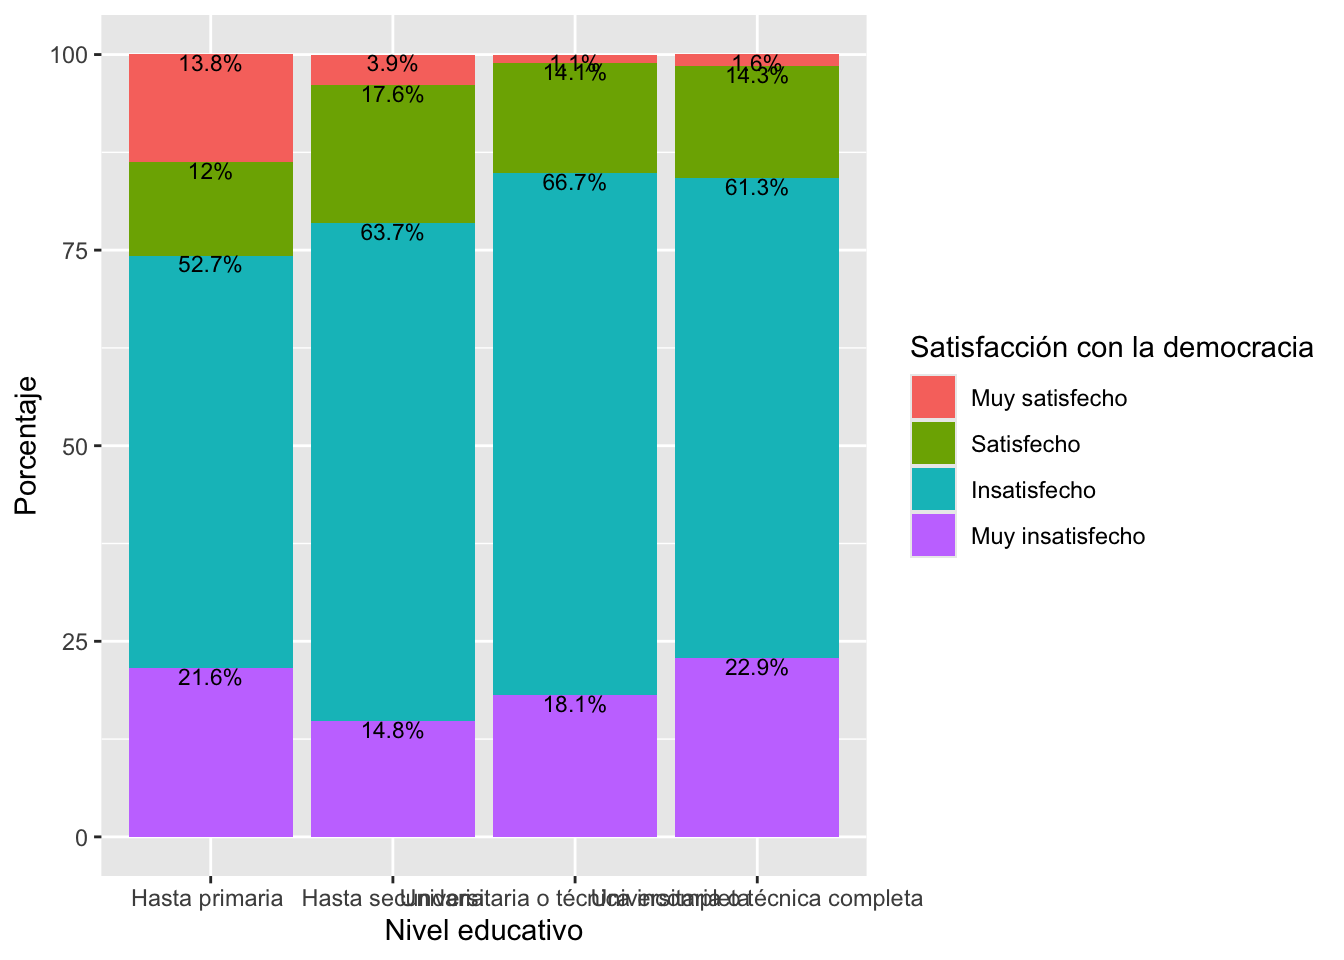
\includegraphics{clase2_files/figure-latex/unnamed-chunk-12-1.pdf}

O con un gráfico de barras.

\begin{Shaded}
\begin{Highlighting}[]
\FunctionTok{hist}\NormalTok{(LL}\SpecialCharTok{$}\NormalTok{education)}
\end{Highlighting}
\end{Shaded}

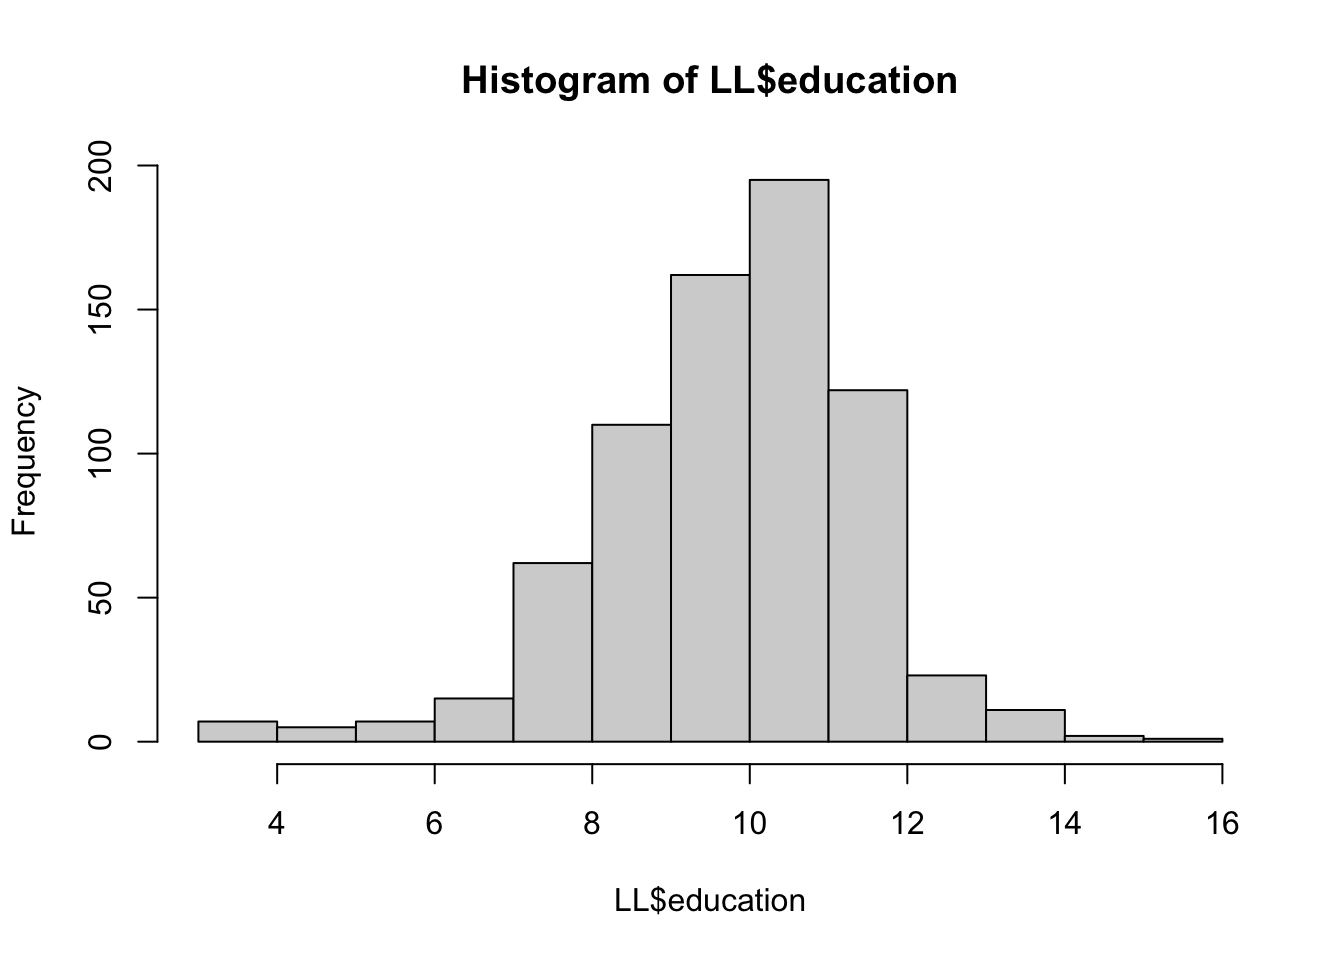
\includegraphics{clase2_files/figure-latex/unnamed-chunk-13-1.pdf}

O mediante

\begin{Shaded}
\begin{Highlighting}[]
\FunctionTok{barplot}\NormalTok{(}\FunctionTok{table}\NormalTok{(LL}\SpecialCharTok{$}\NormalTok{education),}\AttributeTok{xlab=}\StringTok{"Años de educación"}\NormalTok{,}\AttributeTok{ylab=}\StringTok{"Frecuencia"}\NormalTok{,}\AttributeTok{cex.axis=}\NormalTok{.}\DecValTok{9}\NormalTok{,}\AttributeTok{cex.names=}\NormalTok{.}\DecValTok{9}\NormalTok{,}\AttributeTok{ylim=}\FunctionTok{c}\NormalTok{(}\DecValTok{0}\NormalTok{,}\DecValTok{200}\NormalTok{))}
\FunctionTok{abline}\NormalTok{(}\AttributeTok{h=}\DecValTok{0}\NormalTok{,}\AttributeTok{col=}\StringTok{\textquotesingle{}gray60\textquotesingle{}}\NormalTok{)}
\FunctionTok{box}\NormalTok{()}
\end{Highlighting}
\end{Shaded}

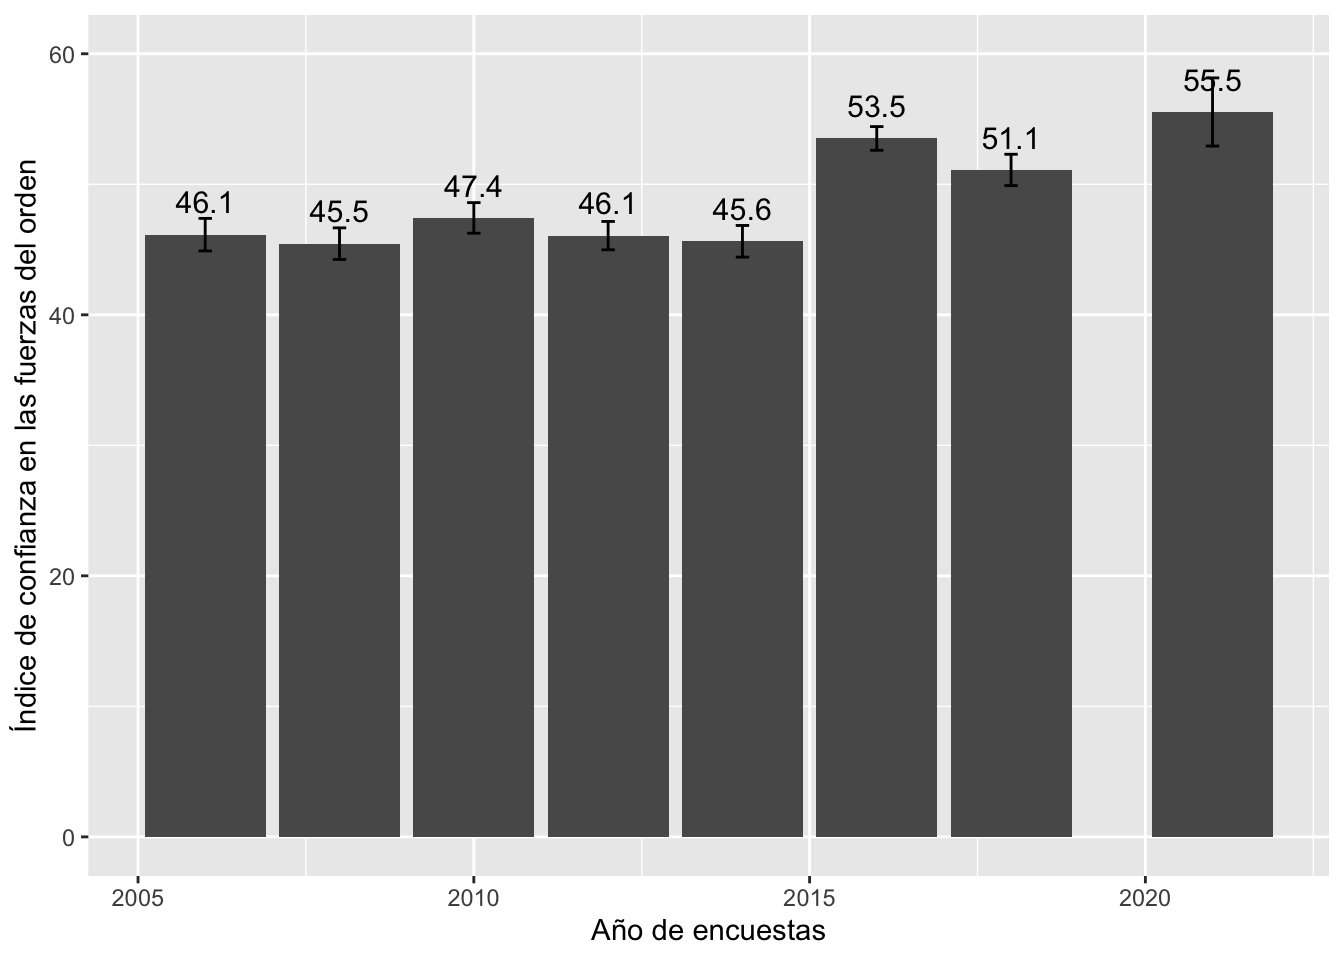
\includegraphics{clase2_files/figure-latex/unnamed-chunk-14-1.pdf}

\hypertarget{medidas-de-dispersiuxf3n-1}{%
\section{Medidas de dispersión}\label{medidas-de-dispersiuxf3n-1}}

\hypertarget{rango-intercuartil-1}{%
\subsection{Rango intercuartil}\label{rango-intercuartil-1}}

Distancia entre Q3 y Q1, que acumula el 50\% de los datos centrales.

\begin{Shaded}
\begin{Highlighting}[]
\FunctionTok{IQR}\NormalTok{(LL}\SpecialCharTok{$}\NormalTok{re74)}
\end{Highlighting}
\end{Shaded}

\begin{verbatim}
## [1] 5211.795
\end{verbatim}

Para una variable numérica, la medida más usada es la desviación
estándar.

\begin{Shaded}
\begin{Highlighting}[]
\FunctionTok{sd}\NormalTok{(LL}\SpecialCharTok{$}\NormalTok{re74)}
\end{Highlighting}
\end{Shaded}

\begin{verbatim}
## [1] 6220.637
\end{verbatim}

¿Calcule una medida de dispersión basada en la mediana?

\hypertarget{inspeccionando-la-hipuxf3tesis-de-lalonde}{%
\section{Inspeccionando la hipótesis de
LaLonde}\label{inspeccionando-la-hipuxf3tesis-de-lalonde}}

Hasta ahora se ha calculado la media de ingresos para el total de los
participantes del estudio en 1974. La idea es analizar cómo cambiaron
estos ingresos entre 1974 y 1978 para cada grupo. Para empezar, ¿cómo
eran los ingresos de los participantes que fueron tratados y que fueron
al grupo control al inicio del estudio? Para esto se tiene que calcular
la media para cada uno de estos grupos. Hay varias maneras de hacer
esto. Una es usando los {[}{]}

\begin{Shaded}
\begin{Highlighting}[]
\FunctionTok{mean}\NormalTok{(LL}\SpecialCharTok{$}\NormalTok{re74[LL}\SpecialCharTok{$}\NormalTok{treated}\SpecialCharTok{==}\DecValTok{0}\NormalTok{])}
\end{Highlighting}
\end{Shaded}

\begin{verbatim}
## [1] 3672.485
\end{verbatim}

\begin{Shaded}
\begin{Highlighting}[]
\FunctionTok{mean}\NormalTok{(LL}\SpecialCharTok{$}\NormalTok{re74[LL}\SpecialCharTok{$}\NormalTok{treated}\SpecialCharTok{==}\DecValTok{1}\NormalTok{])}
\end{Highlighting}
\end{Shaded}

\begin{verbatim}
## [1] 3570.999
\end{verbatim}

Otra opción es creando otros ``dataframes'' para cada grupo con el
comando \texttt{subset}.

\begin{Shaded}
\begin{Highlighting}[]
\NormalTok{trata }\OtherTok{\textless{}{-}} \FunctionTok{subset}\NormalTok{(LL, LL}\SpecialCharTok{$}\NormalTok{treated}\SpecialCharTok{==}\DecValTok{1}\NormalTok{)}
\NormalTok{control }\OtherTok{\textless{}{-}} \FunctionTok{subset}\NormalTok{(LL, LL}\SpecialCharTok{$}\NormalTok{treated}\SpecialCharTok{==}\DecValTok{0}\NormalTok{)}
\end{Highlighting}
\end{Shaded}

Y en cada subgrupo calcular la media. En este caso calcularemos la media
en 1978 para ver si se generaron diferencias.

\begin{Shaded}
\begin{Highlighting}[]
\FunctionTok{mean}\NormalTok{(control}\SpecialCharTok{$}\NormalTok{re78)}
\end{Highlighting}
\end{Shaded}

\begin{verbatim}
## [1] 5090.048
\end{verbatim}

\begin{Shaded}
\begin{Highlighting}[]
\FunctionTok{mean}\NormalTok{(trata}\SpecialCharTok{$}\NormalTok{re78)}
\end{Highlighting}
\end{Shaded}

\begin{verbatim}
## [1] 5976.352
\end{verbatim}

A simple vista, ¿se cumple la hipótesis de LaLonde?

\end{document}
